\subsection{Mean voxels mask}

We plot sample images of the brain from three different perspectives, which 
show how our dataset looks like. Since the paper talks about the noise 
in the data, we average our data by time and plot a histogram to check noise 
variance. The dataset contains a lot of signal noise at the outskirt of the 
brain. The signal in the images extends across several voxels, because nearby 
brain locations usually have similar response to the task. However, the noise 
in the data is mostly independent from one voxel to the next. Therefore, we 
reduce the noise by smoothing in space using averaging across the independent 
noise in the voxels. Based on the histogram, we decide to set the threshold to 
8000 which includes the majority of useless information. Then we extract the data 
points that are larger than 8000 such that all signal noise is removed. Moreover, 
we apply the gaussian filtering to smooth by 2 standard deviation in all three spatial 
dimensions.

\begin{figure}[h]
\centering
\begin{subfigure}{.45\textwidth}
  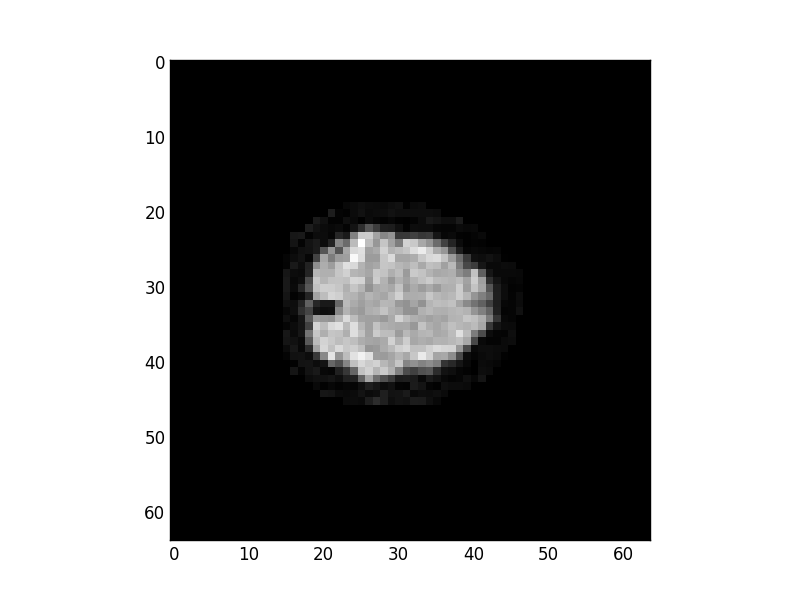
\includegraphics[scale=0.4]{sample_image}
  \caption{Sample Images of Brain}
  \label{fig:sub1}
\end{subfigure}%
\begin{subfigure}{.6\textwidth}
  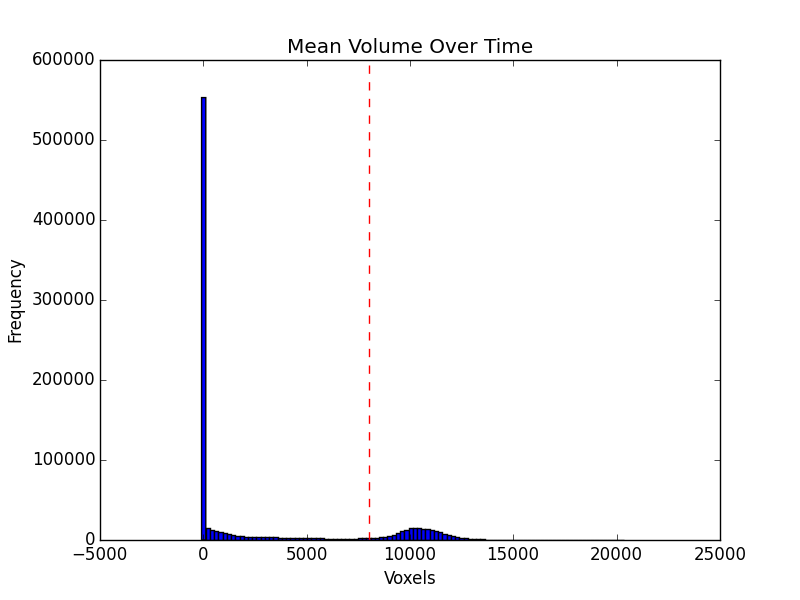
\includegraphics[scale=0.4]{block_mean_data}
  \centering
  \caption{Histogram of Mean of Data}
  \label{fig:sub2}
\end{subfigure}
\end{figure}


